\chapter{The Bracelet}
\label{chap:bracelet}
As presented in the introduction, this thesis aims to design and implement a wrist-worn wearable. Users should interact with it in a casual way, meaning that the interactions are not interrupting the users' current tasks in contrast to typical smartphone interactions that require focus on the display and input. Instead, the frequently used functions for controlling the ambient light should be executed without needing to look at the device, so that additional cognitive and physical load by either social, mental or physical encumbrance does not prevent the user from interacting with the bracelet.

In terms of hardware design, the device should be comfortable to wear, even for a longer period of time. To increase acceptance of potential users, the bracelet should not feel more clumsy than a wristwatch and the material should be skin-friendly. Regarding the interaction design, gestured input as well as a touch sensor that enables sliding interaction need to be included. Although direct feedback of interaction is given by the controlled light source, a minimal form of visual feedback can help the user when in doubt about correctly triggering specific features. In order to communicate with the ambient light, the bracelet needs some form of wireless communication. The device's processor needs to be fast enough to analyze in-air gestures without perceptible delay.

Regarding those constraints, the interactive bracelet consists of several touch sensors, a motion sensor, a status \ac{LED} and a Bluetooth communication module, all powered by an ARM microcontroller. The bracelet's design focuses on wearing comfort, low weight and small error of unintended activation.

\section{Manufacturing Techniques}

All bracelets produced for this thesis were designed using a 3D \ac{CAD} modeler. The first prototypes were 3D printed rigid bodies to wear as armcuffs, but those designs turned out to be too inflexible and uncomfortable to wear. The need for a different material for the bracelets arose, so a transition from printing to casting with liquid silicone took place. The molds are printed, assembled, filled with silicone and usually destroyed while retrieving the finished cast.

This section will explain the various methods and tools used for designing and manufacturing the bracelet prototypes in detail.

\subsection{Computer Aided Design}
%TODO: references
% http://www3.ul.ie/~rynnet/parametricmodellingbasics-solidworks.php
In the beginning of a design iteration, a model of the desired object is created with a 3D \ac{CAD} program. For all designs in this thesis, the open source \ac{CAD} modeler FreeCAD\cite{freecad} was used. This program classifies itself as a general purpose 3D parametric modeler. A typical work-flow when designing a bracelet is as follows:

A bracelet's model is based on a sketch defining the inner circumference of the future bracelet. As the human wrist does not follow a circular shape, all designs made for this thesis are based on an oval circumference. In FreeCAD, this is realized by a composition of arcs and straight lines. It is important to constraint the sketch with radii, lengths and angles as well as symmetries or perpendicular constraints until no degrees of freedom are left and thus the model is fully constrained. If the model is missing some constraints, the export process or the printing of the model can raise errors or alter the design in an unintended way.

In the next step one or more cross sections are added to various points along the circumference. They define the thickness and shape of the bracelet at said points. For increased comfort, the bracelet should be as slim as possible, especially on the ``backside'' below the palm. In more complicated designs, an alternative to complex sketches for the profiles is the creation of multiple, overlaid sketches as a preparation for a subtraction operation in the later process. All profiles need to be fully constrained as well.

\begin{figure}[bth]
	\myfloatalign
	\subfloat[Fully constrained inner circumference]
	{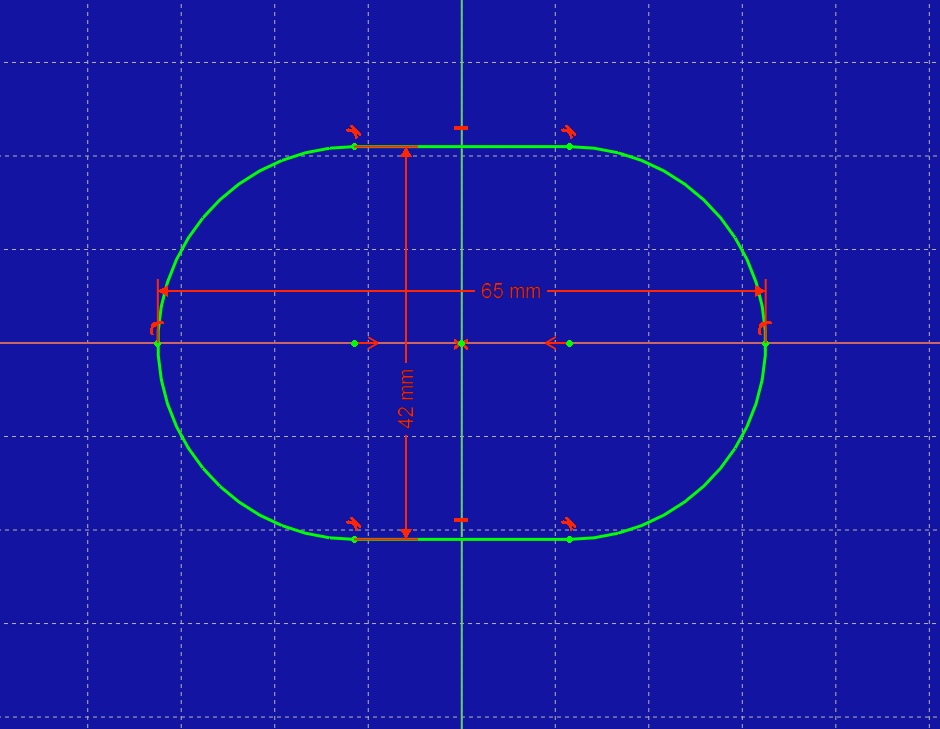
\includegraphics[width=.45\linewidth]{gfx/cad01.png}} \quad
	\subfloat[Added profile for sweeping around the circumference]
	{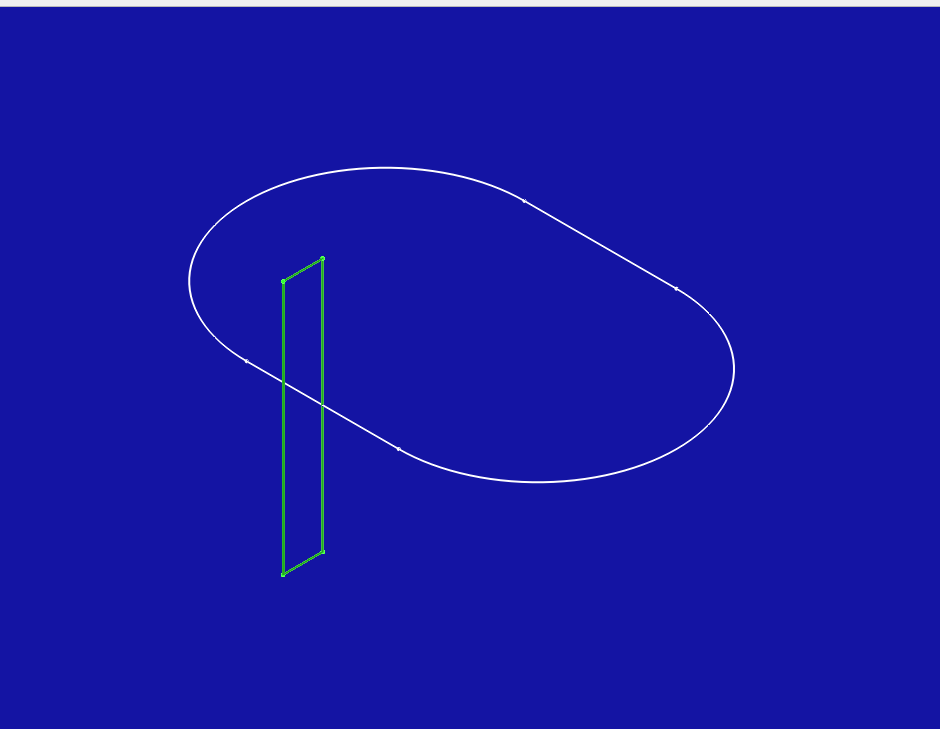
\includegraphics[width=.45\linewidth]{gfx/cad02.png}} \\
	\subfloat[Result after sweeping]
	{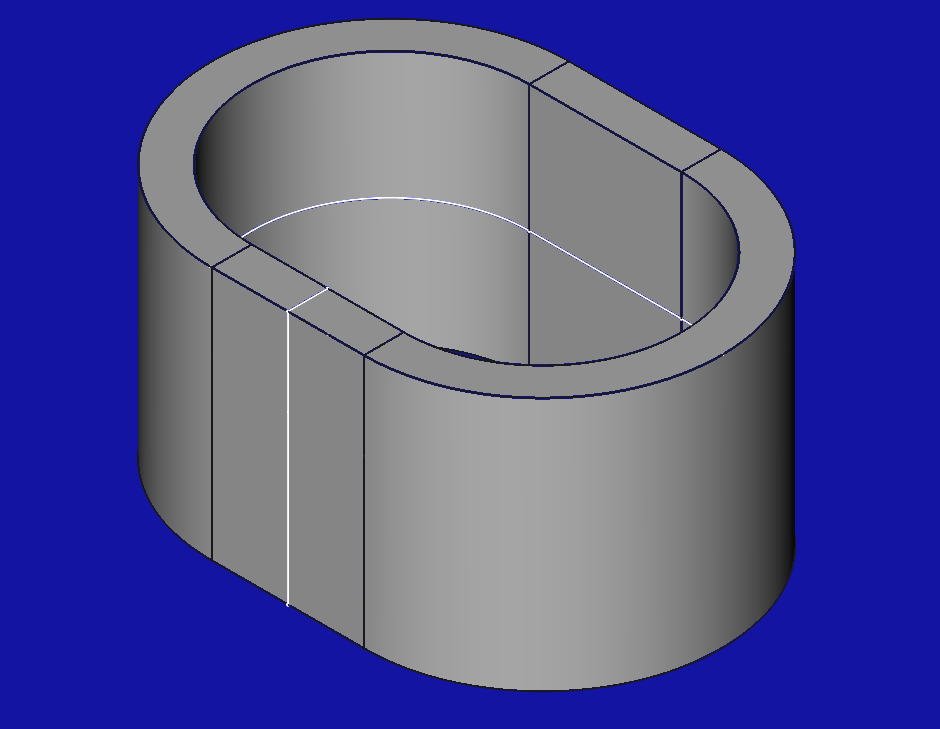
\includegraphics[width=.45\linewidth]{gfx/cad03.png}} \quad
	\subfloat[\ac{CAD} model after using a boolean subtraction operation]
	{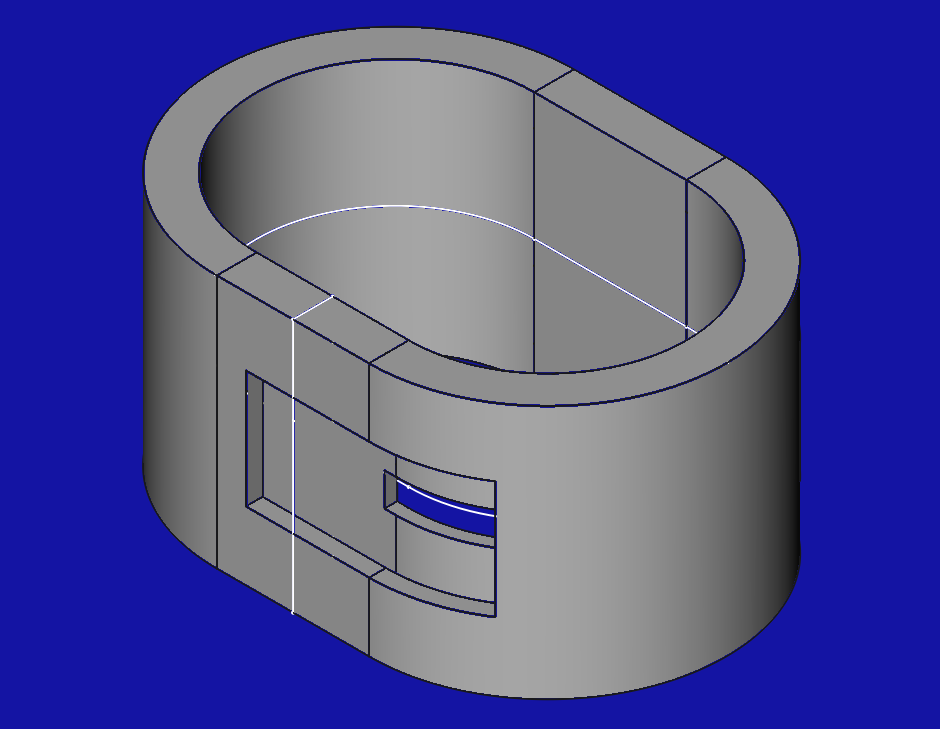
\includegraphics[width=.45\linewidth]{gfx/cad04.png}}
	\caption{Steps in designing a bracelet prototype in FreeCAD.}
	\label{fig:cad}
\end{figure}

After the circumference as well as one or more profiles are added to the design, a first solid is created by sweeping the profile(s) around the circumference curve. This operation creates a basic shape that can be refined further on, typically by chamfering or filleting the edges to increase wearing comfort. If a complex shape is desired, multiple sweeps can be generated and used in boolean operations such as union or subtraction. This is the usual approach for most bracelet designs. Figure \ref{fig:cad} illustrates these steps.

The last step in the design process is usually the finishing of the \ac{CAD} model. In case of the bracelet, this translates to edge smoothing with chamfer or fillet tools. Smoothed edges increase the overall wearing comfort of a bracelet, so they are very desired on edges that contact with the skin.

The finished designs are then exported as mesh files (usually in \ac{STL} format) for printing.

\subsection{3D Printing}
All prints were manufactured using a ProJet360 3D printer\cite{printer}. The model is created by printing the binder fluid onto a plaster-like powder bed in the build area. After each printed layer, a new thin layer of powder is added to the print bed. The ProJet360 allows for a layer thickness of 0.1 mm\cite{datasheet_printer}. This allows even delicate structures without any additional supports, since the printed object is surrounded and therefore supported by plaster powder during the production process. The only drawback of this printing process is that it doesn't support closed, hollow objects since there is no possibility of removing the enclosed excess powder after the process has finished. When designing models for 3D printing, this constraint has to be kept in mind.

The finished object is then carefully removed from the build bed and any excess powder is gently brushed or blown off. The printer offers a cleaning chamber with a pressurized air pistol and a vacuuming system to assist in that task. Without further hardening, the objects are very fragile and easy to break, even with the pressurized air pistol included in the printer. In order to drastically increase the strength of the prints, they are infiltrated with a fluid after they were thoroughly cleaned. Prints produced by the ProJet 360 can be infiltrated with one of three different substances with varying characteristics: The ColorBond "instant-cure infiltrant", the two-part StrengthMax infiltrant "ideal for functional models", and the Salt Water Cure "eco-friendly and hazard-free infiltrant"\cite{datasheet_printer}. All prints produced for this thesis were infiltrated with ColorBond.

The infiltration step adds strength and hardens the material, resulting in a sturdy printed object. However, the objects created with this technique are very rigid and any bending load breaks them easily. Wall strengths of $1.5$ mm and up have been proven sturdy enough for a bracelet shape, although this also depends on the object geometry.

\subsection{Silicone Casting}
%TODO mold making
% http://www.npl.co.uk/science-technology/mass-and-force/hardness/rubber-hardness
% https://www.google.com/patents/US1770045
% http://www.calce.umd.edu/TSFA/Hardness_ad_.htm#3.5
% ISO 7619 for scale OO?
Another manufacturing process for bracelet prototypes used in this thesis is liquid silicone casting. Two different types of silicone were used for making various bracelet prototypes, both from manufacturer Smooth-On: Sorta-Clear 37 and Mold Star 15 Slow.

The most important characteristic for silicone in prototype production is the hardness, measured in Shore (after Albert F. Shore) or Durometer. It measures the indentation of a material with a special device which is also called Shore Durometer. It consists of a hardened steel rod with a finer tip and is available in two versions, since there are two different scales for Shore hardness (cf. table \ref{tab:shore}). The Shore A scale is designed for softer materials and the Shore D scale for harder ones, but they do overlap, so a material classified in Shore D hardness is not necessarily harder than another material classified in Shore A hardness. Each scale ranges from values 0 to 100, higher numbers indicate higher material resistance. The Shore hardness is specified in EN ISO 868.

\begin{table}
	\myfloatalign
	\begin{tabularx}{\textwidth}{clcc} \toprule
		\tableheadline{Type} & \tableheadline{Configuration} & \tableheadline{Diameter} & \tableheadline{Spring Force}\\ 
		\midrule
		A & $35\degree$ & $1.4$ mm & $8.06$ N \\
		D & $30\degree$ & $1.4$ mm & $44.46$ N\\
		OO & $1.2$ mm in spherical radius & $2.4$ mm & $1.11$ N \\
		\bottomrule
	\end{tabularx}
	\caption[Test setups for Shore hardness types]{Test setups for Shore hardness types A, D, and OO \cite{ASTM2240}}  \label{tab:shore}
\end{table}

When dealing with silicone, the Shore A scale is sometimes too "hard" for soft rubbers. Another standard therefore specifies twelve different Durometer types, where the OO scale is commonly used for soft silicones \cite{ISO7619}. Figure \ref{fig:shore} shows the three Shore hardness scales A, D, and OO, as well as some examples for everyday objects and their corresponding Shore values.

\begin{figure}[bth]
	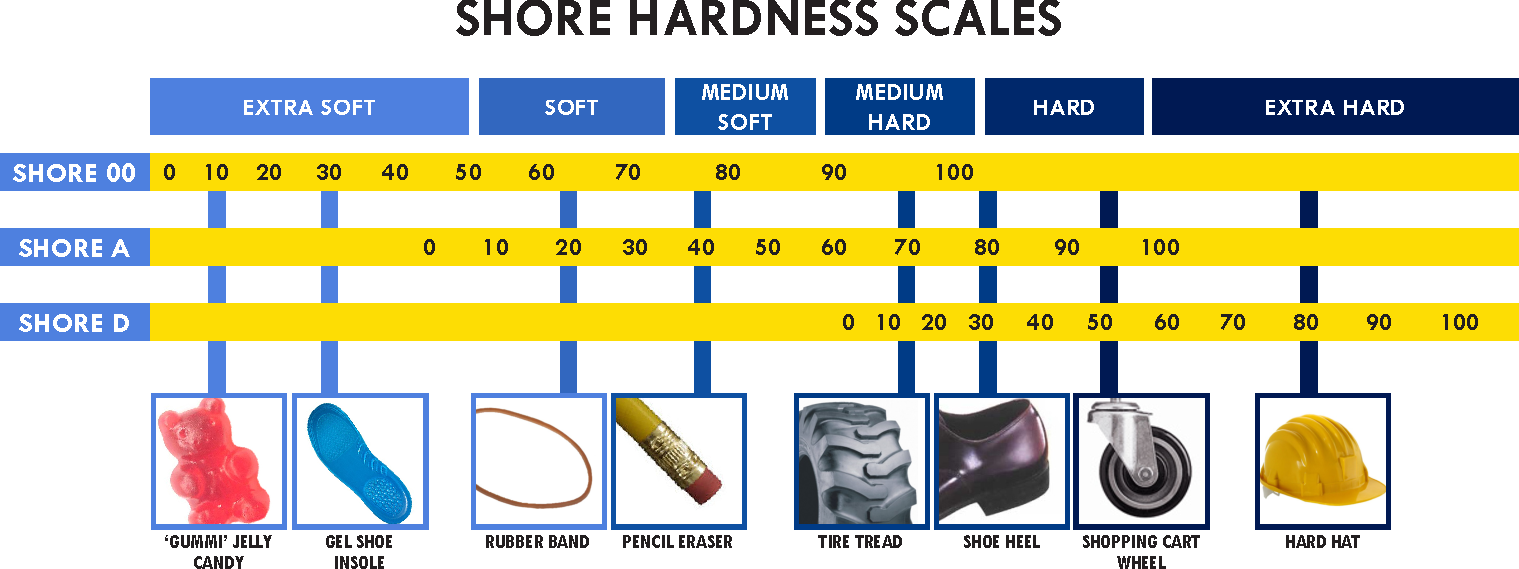
\includegraphics[width=\linewidth]{gfx/durometer_without_logo.pdf}
	\caption[Shore hardness scales and everyday examples]{Shore types A, D, and OO in comparison with everyday examples of various hardnesses. \cite{smoothon-web}}\label{fig:shore}
\end{figure}

The silicone rubbers used for casting bracelet prototypes are both located on the Shore A scale. The softer Mold Star 15 Slow has a Shore A hardness of 15 that could be roughly compared to that of a rubber band according to figure \ref{fig:shore}, while the slightly harder Sorta-Clear 37 has a Shore A rating of 37, similar to that of a pencil eraser \cite{moldstar} \cite{sortaclear}.

Both silicone products consist of two compounds that have to be added up and stirred before casting. While the Mold Star silicone has a rather low viscosity, casting the Sorta-Clear requires careful mold design, since it does not distribute well and is rather viscous. A vibrating table can help in filling the mold completely, but nonetheless were casts with the Sorta-Clear silicone much less fruitful, especially for the detailed molds of the one-piece designs (cf. section \ref{sec:silicone-prototypes}).

\section{Design Process and Prototype Manufacturing}

The design process for the interactive bracelet presented in this thesis went through different stages. At first, a 3D printed casing for the electronics was favored, but turned out to be too inflexible, too fragile and even hindering while worn on the wrist. Later on, a cast silicone bracelet turned out to be more comfortable for the user. The different prototypes are explained in detail in the following sections.

\subsection{Rigid Designs}

The first approach that comes to mind when thinking about bracelet design is a cuff-like, rigid shape. From the\ac{CAD} point of view, the first bracelet prototype consists of a single rectangular profile rotated around a oval curve which was derived from a measured wrist. The bracelet's inside is hollow, in order to store all the electronic components. The cuff's gap was just large enough for the wrist to fit through, although in reality, this lead to light scratches on the skin in combination with the rough texture of the printed material. In addition, the uniform thickness made this first prototype uncomfortable to wear, especially at the open ends. 

To summarize, the uniform thickness made the bracelet feel uncomfortable on the wrist and the material felt unfriendly to the skin. So this fist prototype had some clear downsides that were eliminated in the next iteration.

\begin{figure}[bth]
	\myfloatalign
	\subfloat[\ac{CAD} view]
	{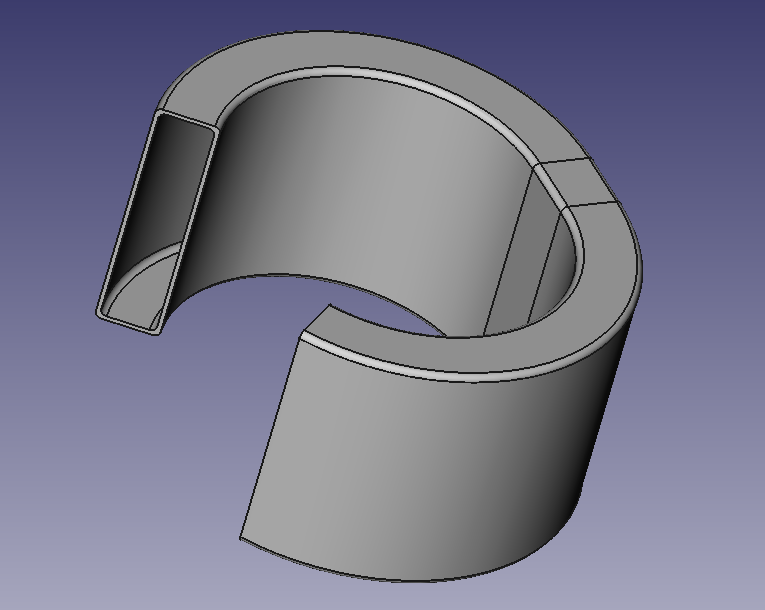
\includegraphics[width=.45\linewidth]{gfx/bracelet01-cad.png}} \quad
	\subfloat[Printed bracelet]
	{\label{fig:bracelet01}%
	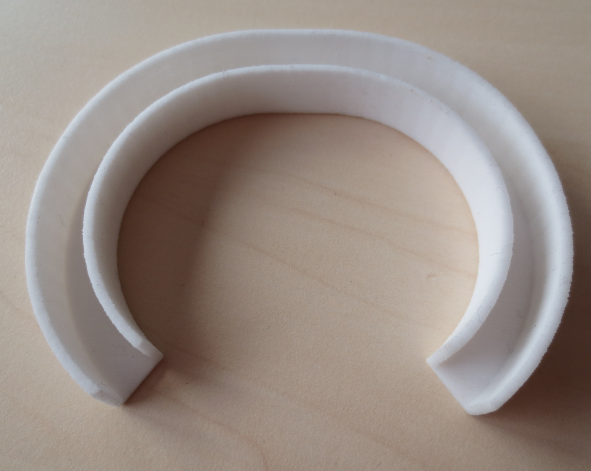
\includegraphics[width=.45\linewidth]{gfx/bracelet01-print-small.png}}
	\caption{First rigid design with uniform thickness}
\end{figure}

In the following iteration, a bracelet of varying thickness was designed to make wearing the prototype more comfortable. The part on top of the wrist was designed to have the highest thickness, since this spot is only rarely disturbing in typical wrist movements and users are likely accustomed to some extra mass on this spot from wearing wristwatches. As the bracelet leads along the arm, its thickness decreases and shrinks to a minimum at the cuff gap. Decreasing the thickness from XX cm to YY cm made the look more appealing and wearing a little less encumbering. At the same time, the wall strength was decreased from X.Y mm to 0.7 mm, which made it very fragile in fabrication and usage, both prints broke during post-processing. Additionally, the possibility of storing electronic components inside the bracelet decreased, since smaller ends featured smaller entrances to the hollow inside. Wearing the cuff while working on a PC felt only slightly uncomfortable, but twisting the hand was still encumbered by the tight-fitting bracelet. 

All in all, a tapered shape felt more comfortable, but the downsides of the material were still present and the improved shape led to less practicability from the engineering point of view. A design goal for future prototypes derived from this prototype was adding more space between the arm and the bracelet to ensure better comfort while wearing it.

\begin{figure}[bth]
	\myfloatalign
	\subfloat[\ac{CAD} view]
	{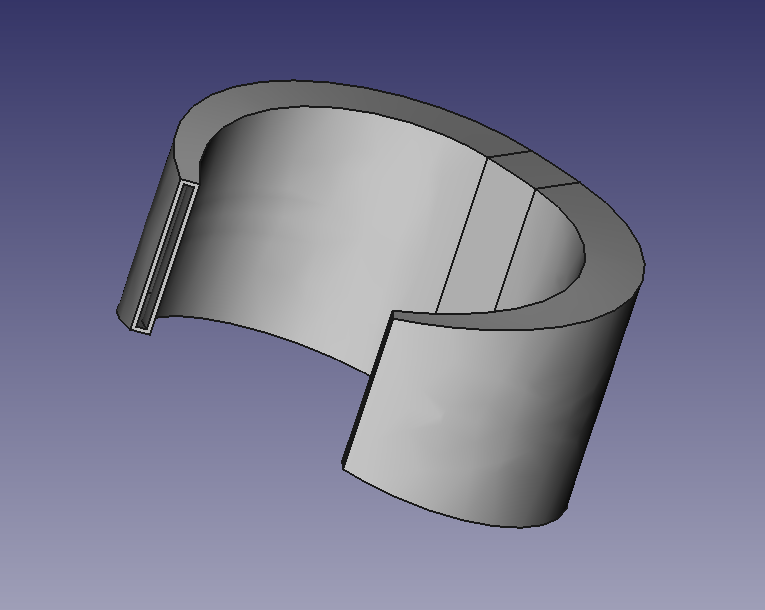
\includegraphics[width=.45\linewidth]{gfx/bracelet02-cad.png}} \quad
	\subfloat[Printed bracelet]
	{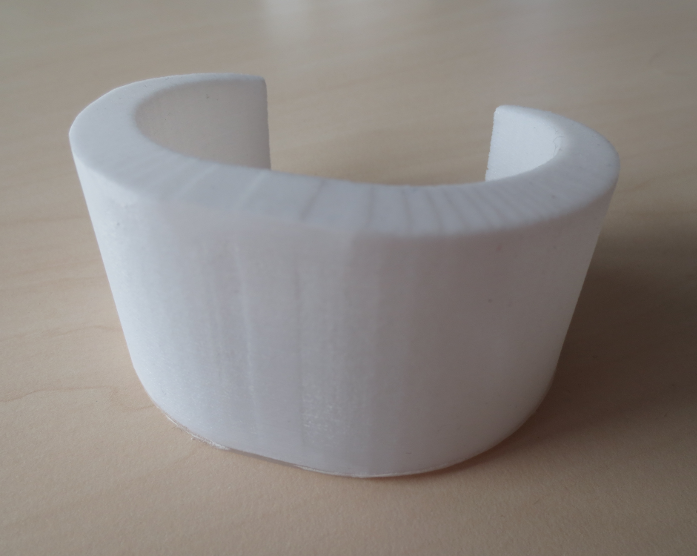
\includegraphics[width=.45\linewidth]{gfx/bracelet02-print-small.png}} \\
	\subfloat[Top view]
	{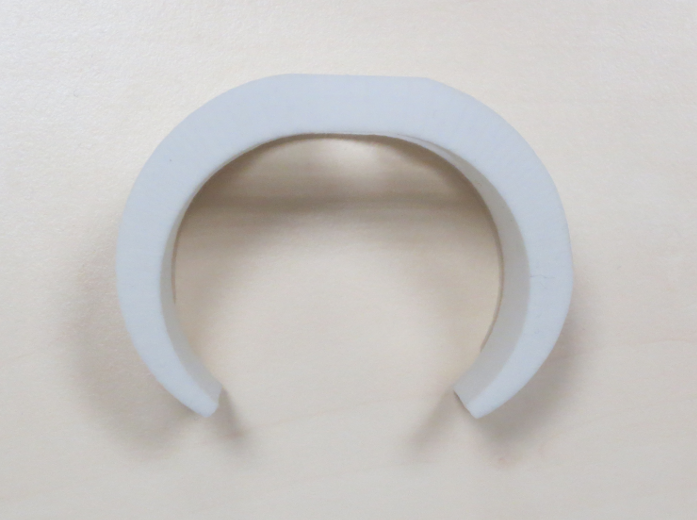
\includegraphics[width=.45\linewidth]{gfx/bracelet02-top.png}} \quad
	\subfloat[End detail]
	{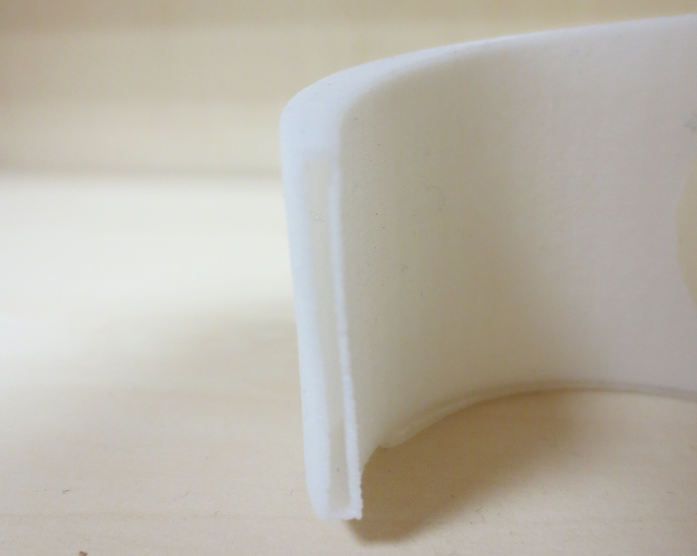
\includegraphics[width=.45\linewidth]{gfx/bracelet02-detail.png}}
	\caption{Second design featuring a tapered shape}
	\label{fig:bracelet02}
\end{figure}

A modified design of the aforementioned prototype featured a removable lid since the tapered shape made it hard to access the inside space of the bracelet. The lid design was inspired by battery case covers commonly found in remote controls or small electronic devices. It features two rabbets on the one side that support the lid in its place and another, smaller rabbet with a cavity in the material right next to it, so the rabbet can snap just inside the lid gap when it closes.

\begin{figure}[bth]
	\myfloatalign
	\subfloat[Lid in \ac{CAD} view]
	{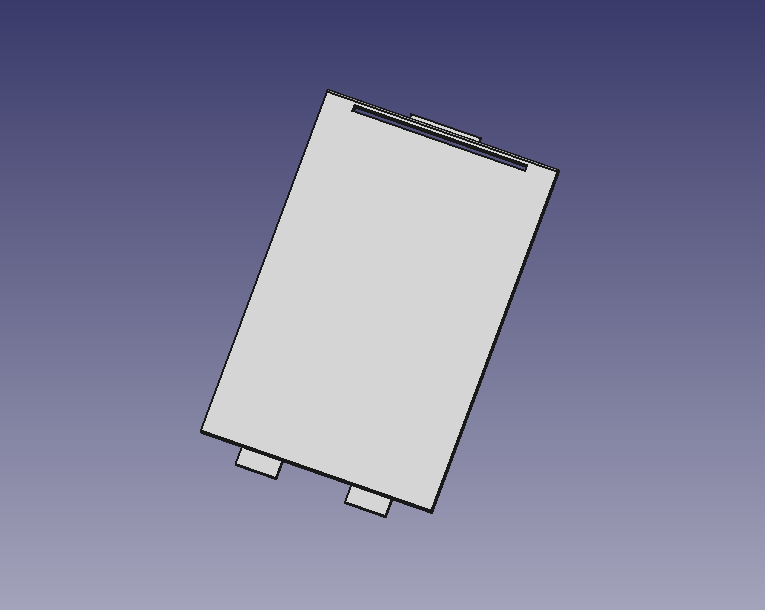
\includegraphics[width=.45\linewidth]{gfx/bracelet03-cad.png}} \quad
	\subfloat[Printed bracelet]
	{\label{fig:bracelet03}%
		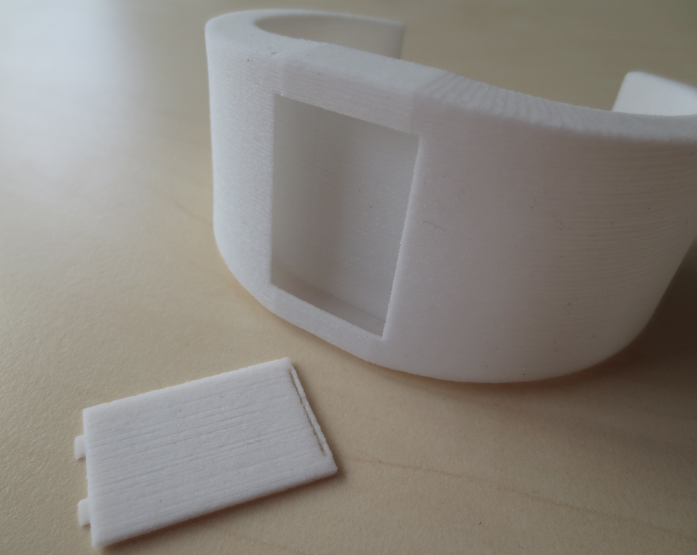
\includegraphics[width=.45\linewidth]{gfx/bracelet03-print-small.png}}
	\caption{Third design with removable lid}
\end{figure}

It turned out that the lid features were designed too fine, especially the flexible part was too thin to work as intended. The lid had to be opened and closed very cautiously and overall, the construction seemed not reliable for daily use. In addition, the rigid shape still lead to clumsiness in wearing the bracelet, so the whole concept of rigid bracelets was left behind.

\subsection{Segmented Designs}

The search for a more flexible printed bracelet shape lead to an entry for an activity bracelet design contest by Daniel Muschke on a 3D printing template exchange site called \textit{GrabCAD} \cite{amicobracelet}. Muschke created a \ac{CAD} file for a bracelet consisting of three segments that are connected by slow hinges, i.e. hinges with great resistance that do not move if no external force is applied. This design considered the electronic components like a micro-controller and a micro \ac{USB} port which made a good start for further modification, but unfortunately the file format made it impossible to alter the design in detail. A print was possible since \ac{STL} files were included in the upload. However, the design turned out to be too small to be actually wearable, but it demonstrated that printed hinges work well with a pivot made from wire. The style felt more comfortable to wear than the previous prototypes and felt leaner on the wrist than the rigid prototypes. Overall, the printed design looked promising so the idea of a multi-part bracelet was investigated further.

Recreating Muschke's design was not as easy as planned, since the parametric modeling approach on this segmented shape was very different in comparison with previous designs. The first prototypes were based on a wrist-like oval circumference curve, while the multi-part design originated from a partitioned circle, since all parts should have the same dimensions in length and curvature. Adjusting the part size to the designated wrist turned out to be difficult, and prints of the design were either too small or too big when printed.

The bracelet segments are hollow and open on the side that lays to the wrist. This leaves enough space for storing electronics. Since the parts are only connected by hinges, routing the necessary wires between the segments needs to be considered, e.g. by leaving small holes right next to the hinges.

\begin{figure}[bth]
	\myfloatalign
	\subfloat[\ac{CAD} view]
	{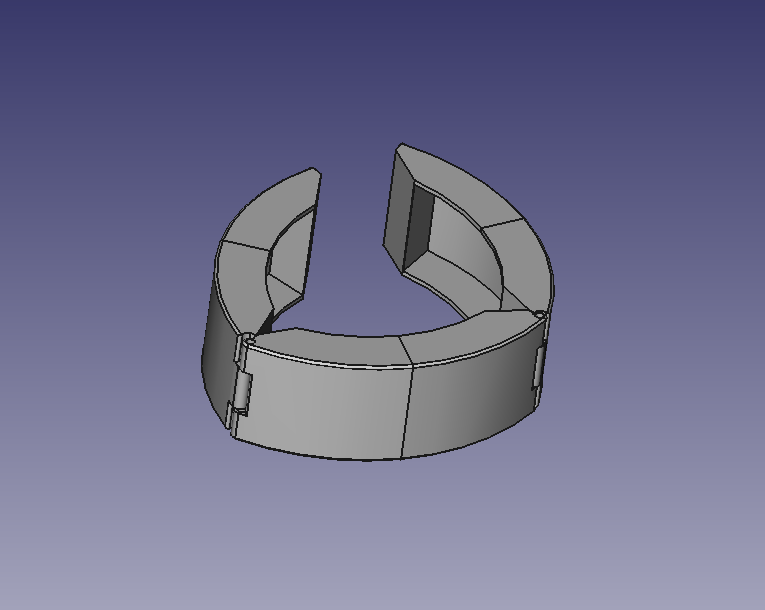
\includegraphics[width=.45\linewidth]{gfx/bracelet04-cad.png}} \quad
	\subfloat[Hinge Detail]
	{\label{fig:bracelet04}%
		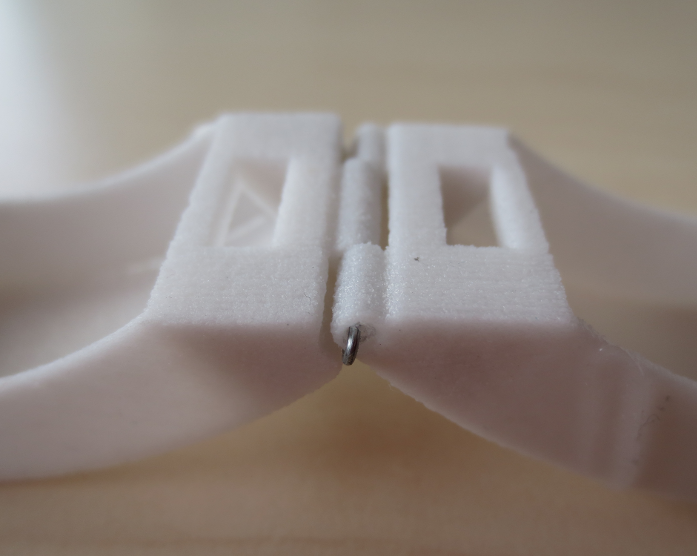
\includegraphics[width=.45\linewidth]{gfx/bracelet04-print-small.png}}
	\caption{Multi-part design}
\end{figure}

Since the manufacturing possibilities at the \ac{HCI} group don't allow for slow hinges (as the inspiration by Muschke suggests), a different solution for keeping the bracelet closed while worn on the wrist needed to be considered. A magnet clasp with small neodymium magnets was tested, but attaching them turned out to be more difficult than expected. When attached to the inside of the segment tips, the magnetic force was too weak for reliably keeping the bracelet together. Mounting the magnets on the outside of the segments resulted in mounting difficulties, since the magnetic force of neodymium magnets is very strong and frequently resulted in torn glue layers.

When an electrophoretic display was considered to be part of the bracelet, the segmented approach became undesired, since in addition to aforementioned difficulties in designing and manufacturing, the usable surface space was relatively small when it came to hosting a single big component like a display. This issue led to further research into various other manufacturing techniques and potential materials for bracelet prototypes, and eventually led to cast silicone.

\subsection{Silicone Bracelet}

After some consideration on a flexible e-ink display, a prototype bracelet made of silicone was considered. The molds used in the casting process were designed and printed just as the bracelets presented in the previous sections. However, designing a mold was significantly more difficult.

As with the previous 3d printed prototypes, the bracelet positive was designed first. The flexibility of silicone allows for some features that weren't practical when implemented in rigid material, for example cavities for electronic components. This resulted in overall more complex bracelet concepts. In addition, closing mechanisms like magnets had to be considered in this design stage.

When the \ac{CAD} process for the positive is finished, the mold is designed by adding surrounding geometries to the model and applying boolean difference operations. If reusability is desired for individual mold components or the whole mold, the geometry and constellation of the mold parts needs to be considered and the characteristics of the printed material have to be taken into consideration. For example, tunnels in the resulting silicone bracelet are not possible if the mold should be usable more than once.

Another important aspect of mold design is planning the casting process. Some types of silicone rubber are more viscous than others, and the mold design needs to make sure that the liquid rubber reaches all corners and delicate parts well. The distribution inside the mold can be supported by applying gentle vibration during the cure process, but this assumes that the liquid silicone is already distributed into most regions of the mold.

The first silicone design was a simple strap with an open pocket for the long electrophoretic display which was considered as a feature of the bracelet at that time in the design process. The closing mechanism relied on molded neodymium magnets for which some cavities were featured in the bracelet design.

Mold design turned out a little tricky but finally succeeded. A two-piece mold was printed which needed a little post-processing to fit properly together. To ensure a proper fit when closed, small tongues and grooves were added too the mold parts. The mold's inside was coated with black spray paint to make it a little smoother, but this didn't work as intended so the painting was omitted in future mold making processes. The filling holes featured for the silicone were too small, and the mixture was more viscous than expected, so the first cast failed and resulted in two small end pieces and nothing in between. Figure \ref{fig:silicone01} (a)-(c) illustrates some steps in this process.

\begin{figure}[bth]
	\myfloatalign
	\subfloat[Unpainted molds]
	{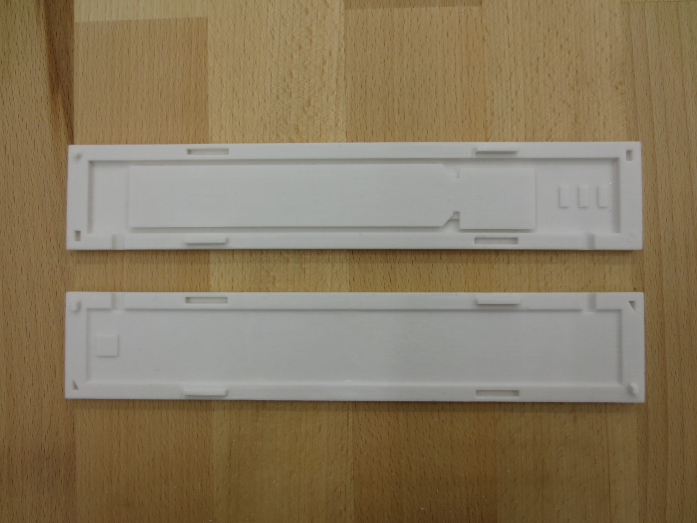
\includegraphics[width=.45\linewidth]{gfx/silicone01-molds.png}} \quad
	\subfloat[Closed molds with filling holes]
	{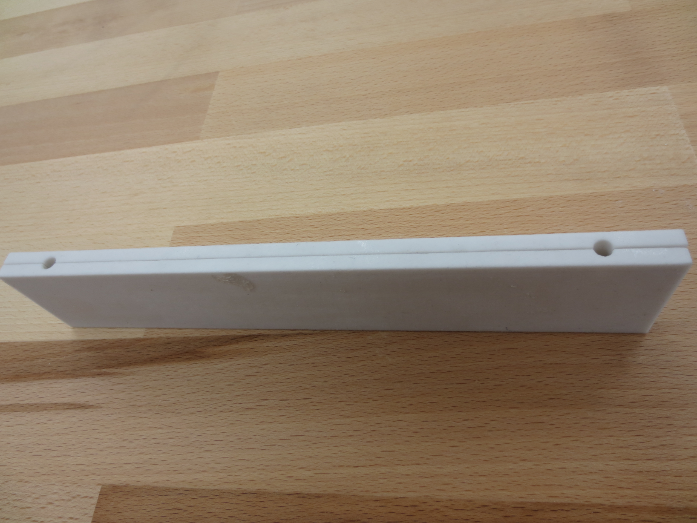
\includegraphics[width=.45\linewidth]{gfx/silicone01-closed.png}} \\
	\subfloat[Result after first cast through filling holes]
	{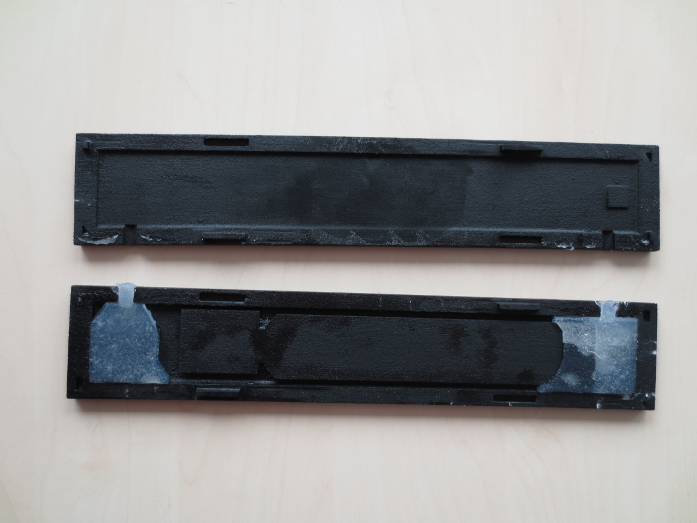
\includegraphics[width=.45\linewidth]{gfx/silicone01-broken.png}} \quad
	\subfloat[Result after second cast by filling the mold directly]
	{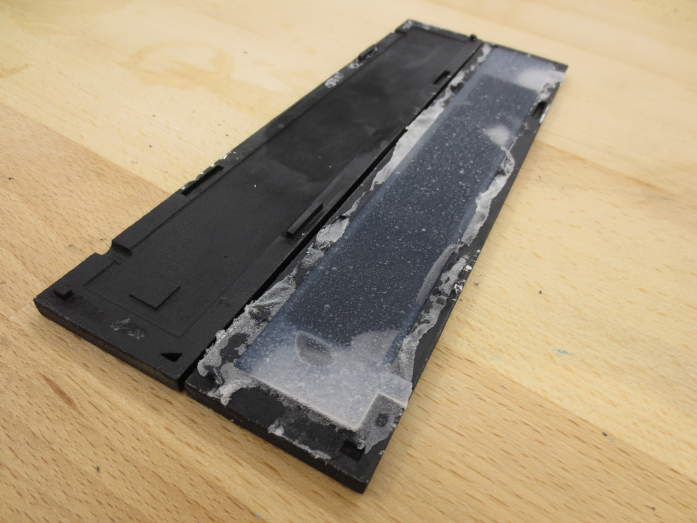
\includegraphics[width=.45\linewidth]{gfx/silicone01-success.png}} \\
	\subfloat[Successfully cast bracelet]
	{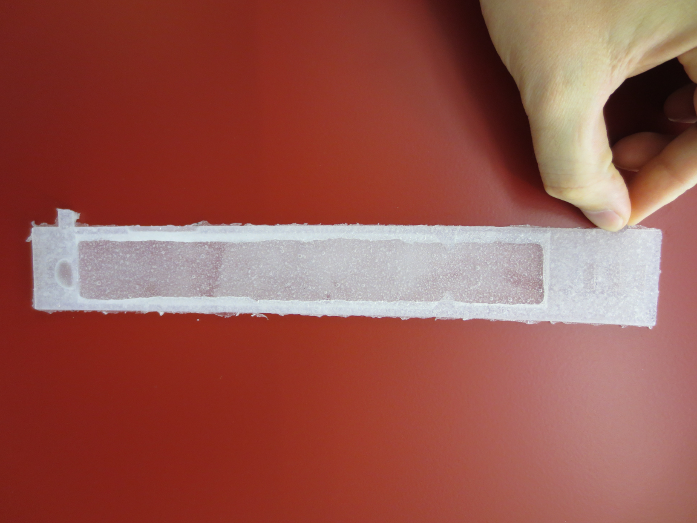
\includegraphics[width=.45\linewidth]{gfx/silicone01-finished.png}} \quad
	\subfloat[Bracelet with attached magnets]
	{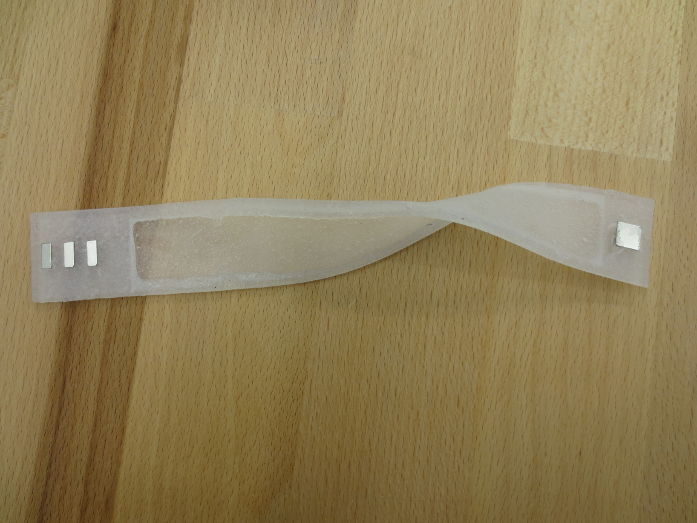
\includegraphics[width=.45\linewidth]{gfx/silicone01-magnets.png}}
	\caption{Manufacturing of a silicone bracelet using a two-piece mold}
	\label{fig:silicone01}
\end{figure}

For following casts, one part of the mold was filled with silicone and closed afterwards; this turned out significantly better (cf. \ref{fig:silicone01} (d)-(e)). The orientation in which the mold is placed during the dry period is also relevant, as air bubbles would float towards the ``top'' of the mold, leading to instabilities when oriented inappropriately. After the liquid silicone's cure period, getting the cast out of its mold was no problem.

This first rubber bracelet design involved a magnet clasp (see fig. \ref{fig:silicone01} (f)), but it was infeasible to reliably attach magnets to silicone with anything but silicone itself and they would likely jump out of place and snap together if placed too close to each other in the design. Apart from that, the silicone felt much more appealing on the skin and was perceived less obstructive while worn on the wrist. The possibility to attach components by placing them in pockets or cavities resulted in thinner bracelets in general.

Two casts were made, one with each of the available silicone mixtures. The softer one was slightly too soft and had a repulsive color. In addition, the cavity rims were too short, so the display would jump out of place almost instantly when bending the bracelet. With this experience and the positive impressions of the material itself, more silicone designs were produced and manufactured.

\subsection{One-Piece Silicone Bracelet}
The next design was a ring-like silicone bracelet in one piece, so the issue with closing mechanisms was no concern. The mold for this prototype consisted of three pieces, an outer and an inner ring as well as a bottom plate to properly align those rings. Due to the very rigid characteristic of the printed material, the molds could not be recovered after the cast and had to be destroyed in order to retrieve the bracelet. In order to prevent unnecessary waste of material, the wall strength was reduced to 2.5 mm which turned out to be strong enough to survive assembly and the casting process. The advantage of using one-time molds was the possibility to add tunnels to the design. This was used in some models, especially for the display area to hide cables or bulky connectors. Figure \ref{fig:bracelethistory} gives an overview on the various design iterations.

\begin{figure}[bth]
	\myfloatalign
	\subfloat[The first design featured a large cavity for a flexible electrophoretic display]
	{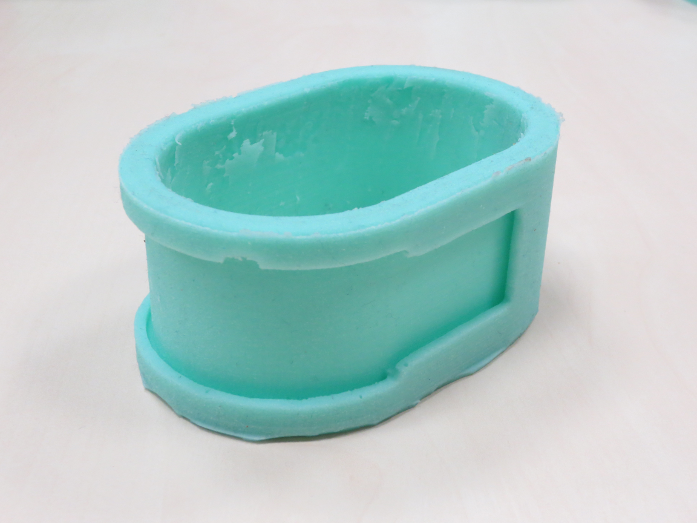
\includegraphics[width=.45\linewidth]{gfx/history01.png}} \quad
	\subfloat[The second design introduced a small tunnel]
	{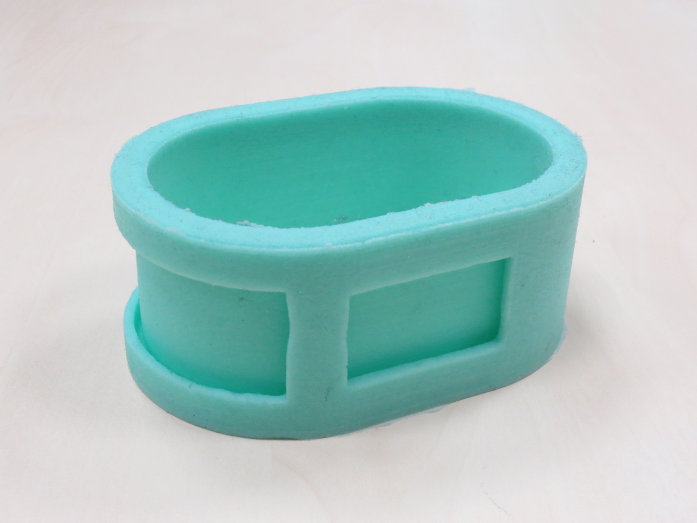
\includegraphics[width=.45\linewidth]{gfx/history02.png}} \\
	\subfloat[The third design replaced the display by a touch strip and featured a cavity for the Teensy]
	{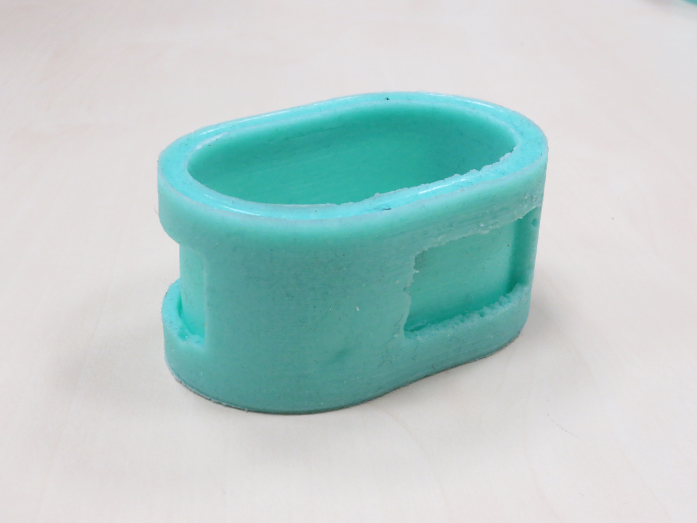
\includegraphics[width=.45\linewidth]{gfx/history03.png}} \quad
	\subfloat[The final design with varying thickness and a big cavity for the Teensy]
	{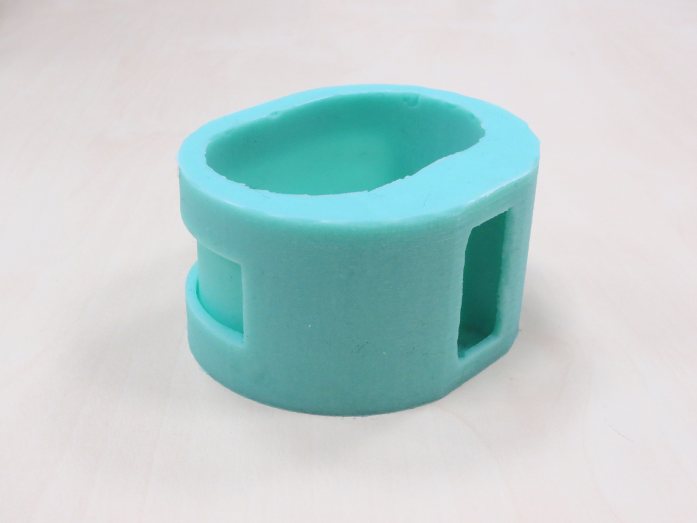
\includegraphics[width=.45\linewidth]{gfx/history04.png}}
	\caption{History of the one-piece bracelet prototyped manufactured for this thesis}
	\label{fig:bracelethistory}
\end{figure}

Those molds were harder to fill with material than the previous one. Especially the Sorta-Clear silicone was too viscous to fill the complete mold, resulting in broken casts. The green MoldStar silicone turned out to work quite well, but sometimes it would leak through little gaps between the rings and the base plate, so a thorough assembly was desired more than ever. Remaining gaps were closed with hot glue in later iterations. In addition, a simple self-made vibrating plate helped filling all parts of the mold and reduced the number of air bubbles in the cast. 

The first one-piece bracelet designs included an electrophoretic display and featured wide cavity rims to hold said display in place. First wearing tests resulted in success. When the display was omitted later on, the cavities stayed to hold a capacitive touch surface in place. After the final hardware configuration took form, another cavity for the electronics was added to the design. Since the hardware was thicker than the bracelet, the spot to house it needed to be enlarged in thickness. The board was eventually placed on the inner wrist and connects to the touch element with a short flat wire cable along the bracelet's surface. It is powered by a micro USB cable attached to a port on the lower rim of the bracelet. A status \ac{LED} is visible through the silicone on the upper rim above the electronics.

\begin{figure}[bth]
	\myfloatalign
	\subfloat[Front view]
	{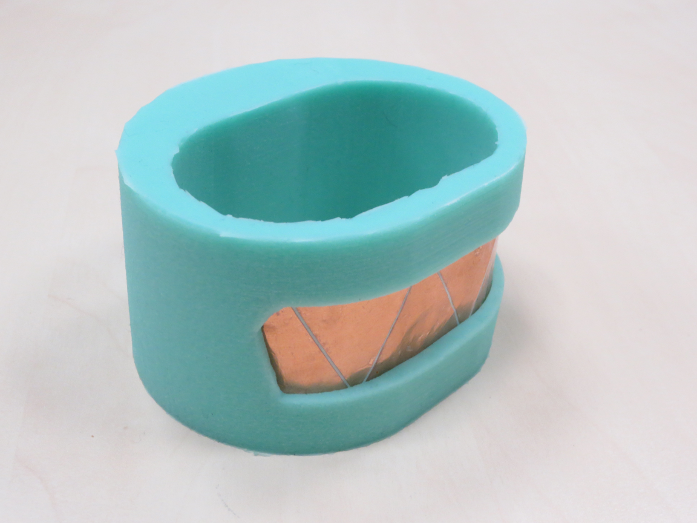
\includegraphics[width=.45\linewidth]{gfx/final-front.png}} \quad
	\subfloat[Back view]
	{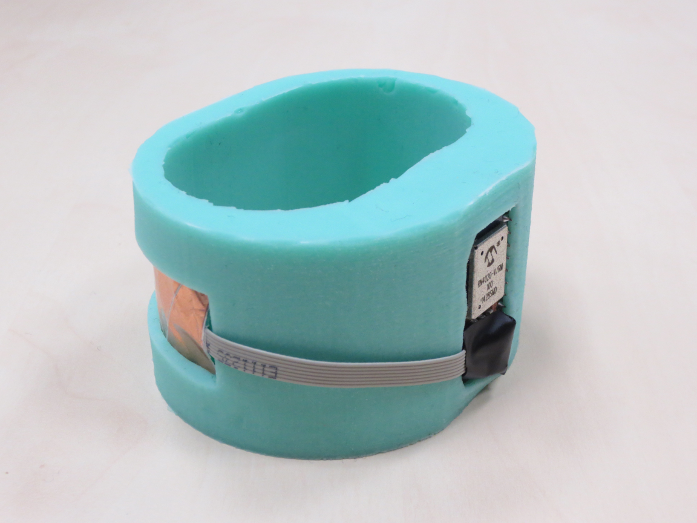
\includegraphics[width=.45\linewidth]{gfx/final-back.png}} \\
	\subfloat[Top view]
	{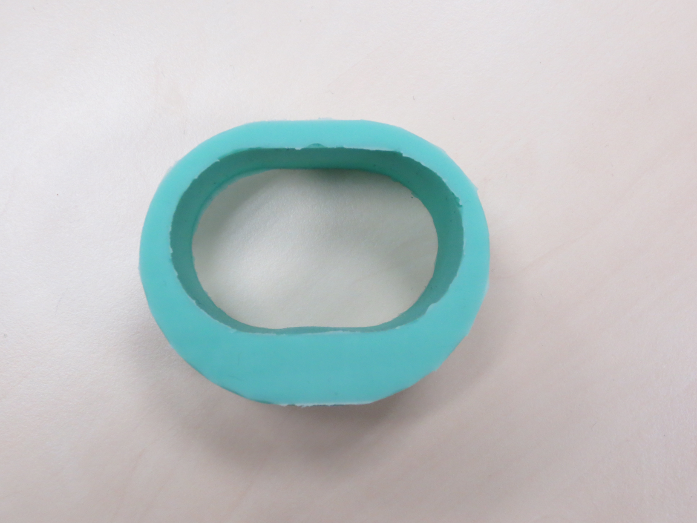
\includegraphics[width=.45\linewidth]{gfx/final-top.png}} \quad
	\subfloat[Incorporated electronics]
	{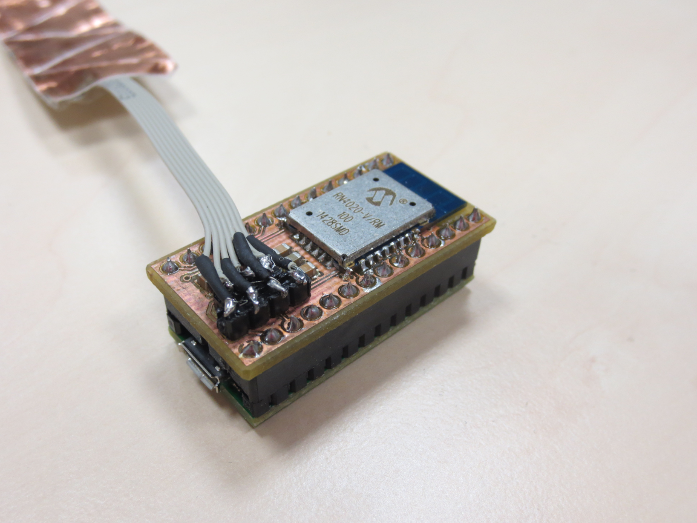
\includegraphics[width=.45\linewidth]{gfx/final-electronics.png}}
	\caption{The final bracelet prototype}
	\label{fig:siliconefinal}
\end{figure}

\section{Teensy Development Board}
The core part of the bracelet's electronics is the Teensy USB development board, which is built around a MK20DX256 32 bit ARM Cortex-M4 Processor running on 72 MHz clock speed \cite{teensy_web}. The Teensy can be programmed using the popular Arduino IDE and thus can profit from the great amount of existing libraries and code examples for the Arduino family.

Like all Cortex processors, the Teensy's chip has direct capability to process capacitive touch input. It also features an \ac{I$^2$C} module for communication with other components (see also section \ref{sec:accel}), several serial communication ports and an integrated programmer to enable flashing via \ac{USB}. However, the processor includes no floating point computation unit, which slows down calculations that feature floating point numbers. %TODO check facts

\section{Touch Slider}
The major input interface of the bracelet is a touch surface which consists of seven cut copper foil segments that are placed in a zigzag pattern. This capacitive strip can either be used as an array of seven individual buttons or as a single large surface that can detect swiping gestures or a primitive variant of multi-touch interaction.

Capacitive touch is based on the concept of a parallel plate capacitor. The copper foil segments act as a capacitor's plate, the human hand touching it represents the other plate. Since the capacitance is proportional to the area of the plates, larger segments lead to increased sensitivity. The definition of a plate capacitor's capacitance $C$ is defined as follows:
\[
	C = \frac{A\epsilon}{d}
\]
Where $A$ represents the area of the plates, $\epsilon$ is a material constant of the dielectric between the plates and $d$ is the distance between the plates. This shows that the capacitance changes more when the finger is close to the sensor and less when it's farther away.

Touch sliders can be compared to a potentiometer and return an analog value for the finger's position on the slider \cite{Camacho2010}. The usual layout of a touch slider features several neighboring electrodes, in the context of this thesis, a slider with seven electrodes was designed and built, since the Teensy has a restricted number of capacitive sensing enables pins from which some were already in use for other components, since almost all pins of the chip serve multiple functions.
%TODO center
\begin{figure}[bth]
	\begin{center}
	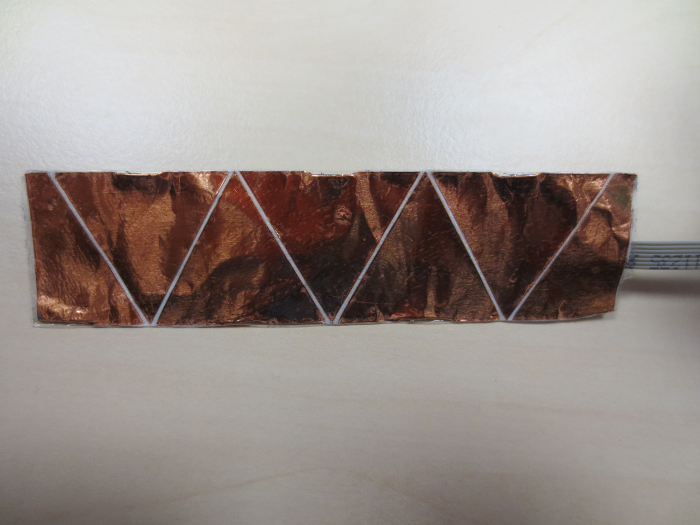
\includegraphics[width=.5\linewidth]{gfx/touchstrip.png}
	\end{center}
	\caption{The capacitive touch strip used in the final bracelet prototype.}\label{fig:touch}
\end{figure}

A zigzagged pattern of the slider's electrodes supports microstepping, i.e. considering the logical combinations of multiple electrodes pressed at the same time to achieve a higher resolution in position detection \cite{Camacho2010}. The touch slider used in this thesis was made using an electronic vinyl cutter with copper tape. The slider is depicted in figure \ref{fig:touch}.

\section{3D Accelerometer}
\label{sec:accel}
Another interaction interface of the bracelet is a MMA8652FC three-axis digital accelerometer \cite{datasheet:mma8652}. In a micromachined device like the one used in this thesis, a seismic mass is attached to delicate "springs" in order to measure the acceleration. Both components are usually made of silicone. When an acceleration occurs, the electric capacitance between the seismic mass and the fixed frame changes and the occurring acceleration can be derived accordingly. Note that one such mechanism is only able to detect acceleration along a single axis. Since the MMA8652FC is a three-axis accelerometer, it contains on mass-spring-system for each of the three axis.
%TODO find better source than (German) wikipedia

\begin{figure}[bth]
	\myfloatalign
	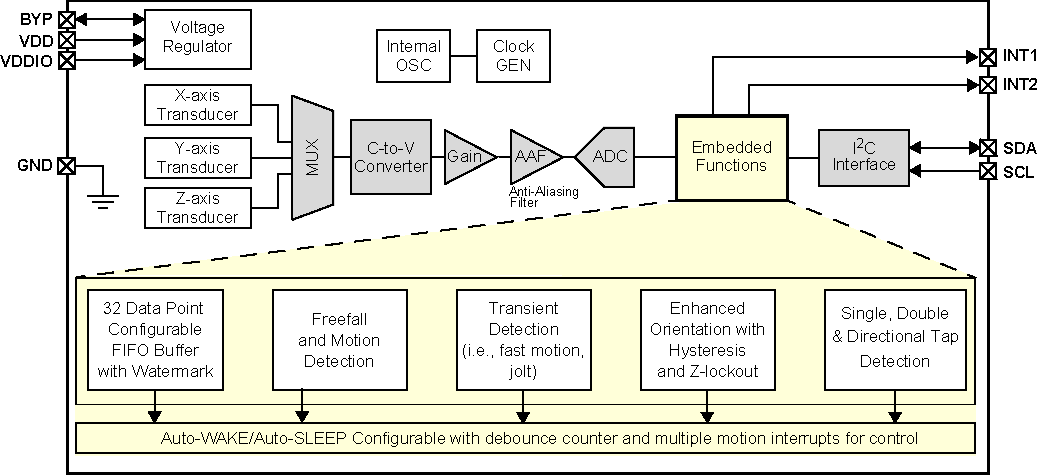
\includegraphics[width=\linewidth]{gfx/accel.pdf}
	\label{fig:accel}
	\caption{Block diagram of the MMA8652FC digital accelerometer. \cite{datasheet:mma8652}}
\end{figure}

In addition to this basic accelerometer functionality, the MMA8652 also features a range of embedded microprocessing functions, as the component's block diagram (fig. \ref{fig:accel}) depicts. Out of those functions, the "Single, Double \& Directional Tap Detection" was used intensively. This module can detect tap interactions, which can be visualized as spikes in the acceleration along one specific axis. The detection process can be configured in detail to adjust factors like the tap intensity or the duration between the two taps of a double tap. When tap detection is enabled, a single register's content indicates if such a tap has occurred. The detailed configuration used for single and double tap recognition in context of this thesis is discussed in section \ref{sec:config}.

In order to communicate with the bracelet's processor, the accelerometer implements the \ac{I$^2$C} communication protocol which was developed in 1982 by Philips Semiconductor (now NXP Semiconductors) and became public domain in 2006 when the underlying patent expired. By using two lines for a clock signal (\textsc{SCL}) and data transmission (\textsc{SDA}) respectively, data can be interchanged in a master-slave system at varying bit rates. Figure \ref{fig:i2c} illustrates this process. To initiate communication, the Teensy incorporates the role of a master device and begins a transmission by changing the \textsc{SDA} value from high to low while \textsc{SCL} is on high. Now the bus is considered busy until the master sends the stop condition and the actual data request and transmission can take place.

\begin{figure}[bth]
	\myfloatalign
	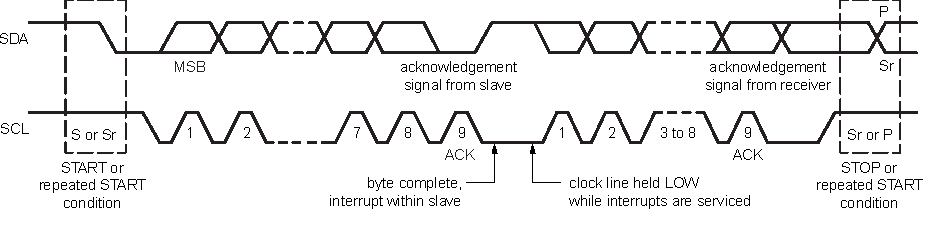
\includegraphics[width=\linewidth]{gfx/i2c.pdf}
	\label{fig:i2c}
	\caption{Data transfer on the \ac{I$^2$C} bus. \cite{i2c}}
\end{figure}

To request register data from the accelerometer, the master writes the address of the desired register on \textsc{SDA}. Note that no further synchronization between master and slave device is needed, since the slave adapts the clock signal on \textsc{SCL} which is determined by the master device. After sending the register's address, the Teensy indicates the end of the transmission without sending a Stop signal. The accelerometer acknowledges the received data and proceeds to send the requested register's contents, and finishes by terminating the connection with a Stop command, which is generated by switching \textsc{SDA} from low to high while \textsc{SCL} is on high. Both lines now stay high due to connected pull-up resistors. If the next register's content is requested, the process starts again with a Start signal transmitted by the master \cite{i2c}.
%TODO verify

\section{Visual Feedback}
To provide visual feedback to the user, an \textsc{RGB} \ac{LED} is incorporated in the bracelet. Since most changes are reflected by the connected light source with no perceptible delay, the \ac{LED} serves mainly as an indicator for the recognition single and double taps in the context of precise color changes and gesture recognition.